\section{The Depth Degradation Atlas}
\label{sec:atlas}

We present the Depth Degradation Atlas: a systematic empirical map of how statistical fingerprints evolve across recursive generation depths, models, and decoding strategies.
The atlas spans $3 \times 3 = 9$ model--strategy cells at the 1--1.5B parameter scale, evaluated at depths $d \in \{0, 1, 2, 3\}$, with depth extensions to $d{=}5$ for cross-model EDD validation (\S\ref{sec:atlas:edd}).

%% ----------------------------------------------------------------
\subsection{In-Distribution Performance}
\label{sec:atlas:id}

Table~\ref{tab:main_matrix} reports four-class Random Forest accuracy (5-fold CV, 200 trees) across all nine cells.
Accuracy ranges from 68.9\% (Pythia, top-$k$) to 85.9\% (GPT-2~XL, temperature) four-class (d1--d3 balanced: 58.9--81.5\%), all exceeding the 25\%/33\% chance baselines.
Two axis effects emerge.
GPT-2~XL achieves the highest accuracy under every strategy (75.8--85.9\%), followed by OLMo (74.4--82.3\%) and Pythia (68.9--78.7\%).
Top-$k$ sampling yields the lowest accuracy in every model.
The mean within-model strategy gap is 9.3~pp, comparable to the 7.2~pp mean within-strategy model gap; decoding strategy contributes at least as much as model family to performance variance.

\begin{table}[t]
\centering
\small
\caption{Four-class RF accuracy (\%) with bootstrap 95\% CI (${\pm}$half-width; $B{=}10{,}000$). RF with 200 trees, evaluated via 5-fold stratified CV (seed=42). Parenthesized: d1--d3 balanced accuracy from the same 4-class RF (chance = 25\% / 33\%). Depth-0 recall exceeds 97\% in all cells. Within-distribution ordinal quality: mean absolute error (MAE)\,=\,0.23, QWK\,=\,0.89 (QWK$_{\text{d1--d3}}$\,=\,0.74); 98.2\% of errors fall on adjacent depths ($|\Delta| \leq 1$). $^\dagger$Self-reference scoring (Pythia-1.4B is both generator and reference model); 4--11\,pp advantage over cross-model references (Appendix~\ref{app:ref_ablation}). Cross-cell comparisons involving Pythia should be interpreted with this caveat.}
\label{tab:main_matrix}
\resizebox{\columnwidth}{!}{%
\begin{tabular}{@{}lccc@{}}
\toprule
& Nucleus & Temp.\ $\tau{=}0.9$ & Top-$k$ \\
\midrule
Pythia-1.4B$^\dagger$  & 78.7{\scriptsize$\pm$0.5}\,(71.8) & 76.8{\scriptsize$\pm$0.5}\,(69.3) & 68.9{\scriptsize$\pm$0.6}\,(58.9) \\
OLMo-1B     & 78.9{\scriptsize$\pm$0.5}\,(72.7) & 82.3{\scriptsize$\pm$0.5}\,(76.6) & 74.4{\scriptsize$\pm$0.5}\,(66.2) \\
GPT-2~XL    & \textbf{84.3}{\scriptsize$\pm$0.5}\,(79.6) & \textbf{85.9}{\scriptsize$\pm$0.5}\,(81.5) & \textbf{75.8}{\scriptsize$\pm$0.6}\,(68.1) \\
\bottomrule
\end{tabular}}
\end{table}

\paragraph{Per-class recall.}
Depth-0 recall exceeds 97\% in all 9 cells.
Among generated depths, d2 consistently yields the lowest recall (44--73\%), reflecting its position at the center of the depth gradient where features overlap with both d1 and d3, consistent with d2-vs-d3 as the EDD bottleneck (\S\ref{sec:atlas:edd}; full per-class recall in Appendix~\ref{app:per_class}).

%% ----------------------------------------------------------------
\subsection{Feature Consistency Across the Grid}
\label{sec:atlas:features}

Multicollinearity is substantial (VIF${>}$10 for 14--16 of 19 features); importance rankings below indicate feature \emph{family} contributions rather than individual effects; permutation importance (Appendix~\ref{app:permutation}) partially mitigates collinearity bias \cite{strobl2008_conditional,hooker2021_permutation}.
Despite the 17.0~pp accuracy spread across cells, the perplexity tail statistics family (\texttt{p90\_ppl}, \texttt{p75\_ppl}, \texttt{kurtosis\_ppl}) and surprisal variance (\texttt{var\_surprisal}) dominate depth discrimination in every setting.
Within this family, \texttt{p90\_ppl} and \texttt{var\_surprisal} are consistently prominent, though individual rankings should be interpreted cautiously given VIF${>}$10; group-level ablation (\S\ref{sec:atlas:features}, below) provides the collinearity-robust confirmation.\footnote{The group-level dominance of perplexity tail statistics is robust across importance measures (Gini, SHAP, permutation; Kendall's $W{=}0.90$, $p{<}0.005$).}
Conditional permutation importance \citep{strobl2008_conditional} confirms \texttt{var\_surprisal} and \texttt{p90\_ppl} as top-2 in 8/9 cells (bootstrap rank 1.4 and 1.7), consistent with Gini rankings (Appendix~\ref{app:conditional_pi}).
Table~\ref{tab:feature_importance} shows the full per-cell ranking; Figure~\ref{fig:atlas_heatmap} visualizes the importance landscape across all nine cells.

Cross-model feature-rank Spearman correlation averages $\bar{\rho} = 0.868$ ($[0.619, 0.954]$): models agree on which features carry depth information despite differing in absolute accuracy.
Top-$k$ yields the highest cross-model rank correlation ($\rho = 0.811$), as vocabulary truncation imposes a more uniform feature landscape at the cost of weaker signal (\S\ref{sec:atlas:strategy}).

Feature ablation confirms this concentration: the top-5 features achieve 97.6\% of full accuracy (76.5\% vs.\ 78.4\%); in-distribution group-level ablation shows perplexity features alone reach 76.6\%, surprisal 73.2\%, lexical diversity ${\leq}$47\%, and repetition ${\leq}$44\% (Appendix~\ref{app:feature_ablation}).\footnote{Best single feature (\texttt{p90\_ppl}) achieves 58.3\%, providing a more competitive single-feature baseline than mean perplexity (25.1\%).}

The feature hierarchy shifts with depth.
At shallow boundaries (d1 vs.\ d2), \texttt{var\_surprisal} dominates importance; at deeper boundaries (d3 vs.\ d4, d4 vs.\ d5), tail perplexity statistics (\texttt{p90\_ppl}, \texttt{kurtosis\_ppl}) take over.
This transition aligns with model-collapse dynamics~\cite{shumailov2024_nature}: early recursion narrows the surprisal distribution (captured by its variance), while later steps erode the perplexity tail (captured by upper quantiles and kurtosis).

\begin{table}[t]
\centering
\small
\caption{Top-5 features by Gini importance. \textbf{Bold}: top-2. \texttt{p90\_ppl} top-2 in 9/9; \texttt{var\_surprisal} 8/9 under SHAP (7/9 under Gini). Individual rankings are approximate due to multicollinearity (VIF${>}$10 for 14--16/19 features).}
\label{tab:feature_importance}
\resizebox{\columnwidth}{!}{%
\begin{tabular}{@{}l l@{}}
\toprule
Cell & Top-5 features (Gini importance, ranked) \\
\midrule
Pythia, nuc.       & \textbf{var\_surprisal\,(.17)}, \textbf{p90\_ppl\,(.15)}, mean\_ppl\,(.11), var\_ppl\,(.08), p75\_ppl\,(.07) \\
Pythia, $\tau$     & \textbf{var\_surprisal\,(.17)}, \textbf{p90\_ppl\,(.14)}, mean\_ppl\,(.11), p75\_ppl\,(.07), mean\_surprisal\,(.07) \\
Pythia, top-$k$    & \textbf{var\_surprisal\,(.16)}, \textbf{p90\_ppl\,(.12)}, mean\_ppl\,(.11), var\_ppl\,(.07), mean\_surprisal\,(.06) \\
GPT-2\,XL, nuc.    & \textbf{var\_surprisal\,(.21)}, \textbf{p90\_ppl\,(.21)}, p75\_ppl\,(.10), mean\_surprisal\,(.07), mean\_ppl\,(.06) \\
GPT-2\,XL, $\tau$  & \textbf{p90\_ppl\,(.25)}, \textbf{p75\_ppl\,(.15)}, mean\_surprisal\,(.13), var\_surprisal\,(.12), p50\_ppl\,(.05) \\
GPT-2\,XL, top-$k$ & \textbf{p90\_ppl\,(.24)}, \textbf{p75\_ppl\,(.12)}, var\_surprisal\,(.10), mean\_surprisal\,(.09), type\_token\_ratio\,(.04) \\
OLMo, nuc.         & \textbf{p90\_ppl\,(.18)}, \textbf{var\_surprisal\,(.15)}, p75\_ppl\,(.11), mean\_surprisal\,(.07), type\_token\_ratio\,(.06) \\
OLMo, $\tau$       & \textbf{p90\_ppl\,(.21)}, \textbf{var\_surprisal\,(.16)}, p75\_ppl\,(.12), mean\_surprisal\,(.09), type\_token\_ratio\,(.05) \\
OLMo, top-$k$      & \textbf{p90\_ppl\,(.20)}, \textbf{var\_surprisal\,(.17)}, p75\_ppl\,(.10), mean\_surprisal\,(.07), mean\_ppl\,(.05) \\
\bottomrule
\end{tabular}}
\end{table}

\begin{figure}[t]
\centering
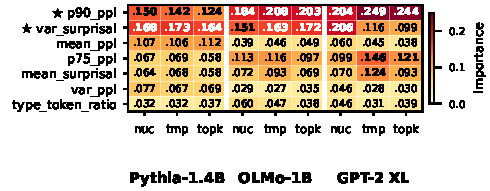
\includegraphics[width=\columnwidth]{figures/fig_atlas_heatmap.pdf}
\caption{Atlas feature importance heatmap for the top-7 features. Rows: features ranked by mean Gini importance; columns: 9 model--strategy cells. Stars mark the two universal top-2 features (\texttt{p90\_ppl}, \texttt{var\_surprisal}). Feature group ablation in Appendix~\ref{app:feature_ablation}.}
\label{fig:atlas_heatmap}
\end{figure}

%% ----------------------------------------------------------------
\subsection{EDD Analysis}
\label{sec:atlas:edd}
\label{sec:atlas:monotonicity}

Depth features exhibit strong monotonic trends (Spearman $\rho = -1.0$ for perplexity tail statistics; Figure~\ref{fig:feature_trajectory}); inter-depth distances are non-uniform (d0-vs-d1 AUC ${>}$0.98 in all 9 cells, d2-vs-d3: 0.69--0.88).

\begin{figure*}[t]
\centering
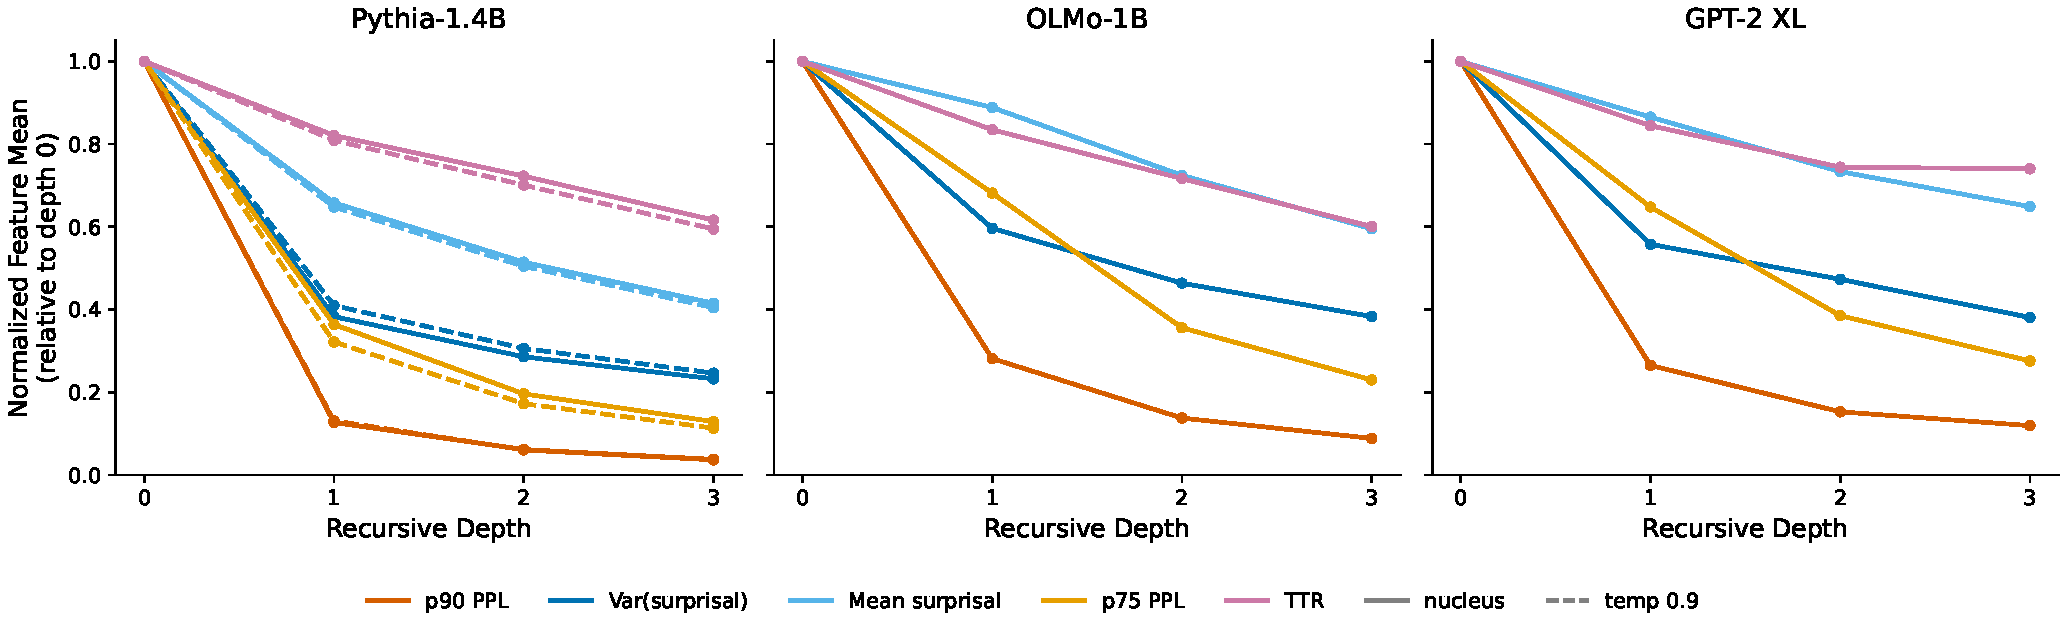
\includegraphics[width=0.78\textwidth]{figures/fig_feature_trajectory.pdf}
\caption{Feature trajectories (normalized to depth~0) across models and strategies. The $d{=}0 \to d{=}1$ gap dominates; tail features (\texttt{p90\_ppl}, \texttt{p75\_ppl}) decline most steeply, consistent with tail erosion (\S\ref{sec:method:theory}).}
\label{fig:feature_trajectory}
\end{figure*}

We extend the benchmark to depth $d{=}5$ for all three models under nucleus sampling.
Each model's depth-3 LoRA checkpoint is used to finetune and generate depth-4 data, and the process repeats for depth~5; feature extraction uses the same reference model (Pythia-1.4B).
We train dedicated binary RF classifiers (500 trees) for each adjacent pair, as defined in Eq.~\ref{eq:edd}.

\paragraph{AUC decay and cross-model convergence.}
For Pythia-1.4B (nucleus), AUC decays monotonically from $0.999$ (d0v1) to $0.683$ (d4v5); AUC-excess contraction ratios (0.80 at d1v2$\to$d2v3, 0.69 at d3v4$\to$d4v5) show convergence toward indistinguishability accelerates with depth (Figure~\ref{fig:auc_decay}).
The d3-vs-d4 AUC clusters near $T{=}0.75$ for all three models (Pythia $0.784$, OLMo $0.765$, GPT-2~XL $0.750$), while d4-vs-d5 converges to a narrow band ($0.681$--$0.684$, range $0.003$), suggesting an architecture-independent depth ceiling within the 1--1.5B nucleus setting.
Bootstrap testing ($H_0{:}\, \mathrm{AUC} \leq 0.75$; Bonferroni-corrected for 3 comparisons, $\alpha{=}0.0167$) yields $p = 0.001$ (Pythia), $0.091$ (OLMo), $0.505$ (GPT-2~XL).

\paragraph{EDD threshold sensitivity.}
Across the 9-cell benchmark (depths 0--3), all cells achieve $\mathrm{EDD}{=}3$ at $T{=}0.65$; at $T{=}0.70$, 8/9 cells; at $T{=}0.75$, 7/9; at $T{=}0.80$, 5/9.
Top-$k$ configurations lose $\mathrm{EDD}{=}3$ first (Pythia top-$k$ at $T{=}0.70$, OLMo top-$k$ at $T{=}0.75$); d2-vs-d3 is the consistent bottleneck.

\begin{figure}[t]
\centering
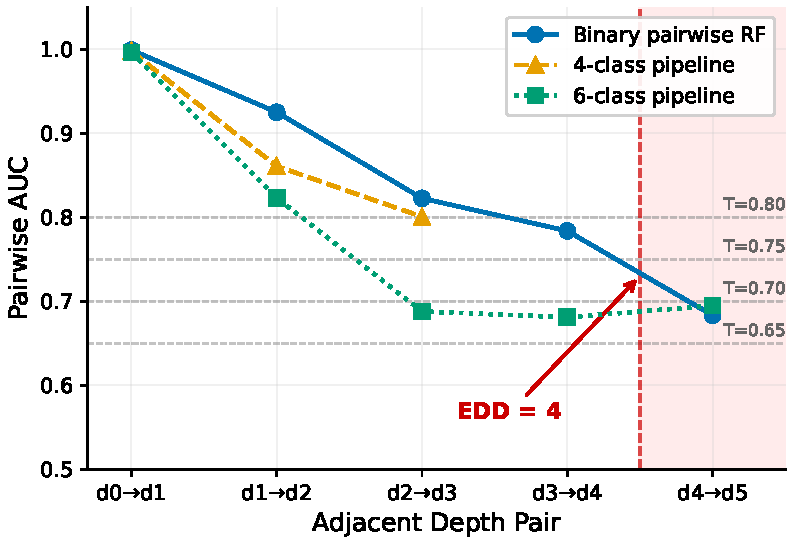
\includegraphics[width=\columnwidth]{figures/fig_auc_decay.pdf}
\caption{AUC decay curves for Pythia-1.4B (nucleus, depths 0--5) under three pipeline configurations: binary pairwise RF, 4-class RF, and 6-class RF. Horizontal dashed lines mark $T \in \{0.65, 0.70, 0.75, 0.80\}$. All curves converge below 0.70 at d4-vs-d5. Shaded bands: bootstrap 95\% CIs.}
\label{fig:auc_decay}
\end{figure}

%% ----------------------------------------------------------------
\subsection{Strategy-Dependent Trajectories}
\label{sec:atlas:strategy}

The three strategies induce qualitatively distinct degradation trajectories.
Temperature ($\tau{=}0.9$) yields the highest accuracy in 2/3 models (GPT-2~XL 85.9\%, OLMo 82.3\%) because uniform logit scaling accelerates convergence to an attractor~\cite{shumailov2024_nature}, amplifying the fingerprint but creating a boundary reversal risk under cross-strategy transfer (\S\ref{sec:generalization}).
Top-$k$ ($k{=}50$) produces the lowest accuracy (68.9--75.8\%) because hard vocabulary truncation removes depth-discriminative low-probability tokens.
The strategy effect (9.3\,pp range) exceeds the model effect (7.2\,pp); deployment-time knowledge of the decoding strategy matters at least as much as the generator model.
